\chapter{Event-based Model}
\label{chapter:ebm}

\newcommand{\scaleF}{0.6}

In this chapter we present analysis that has been done with the event-based model on the DRC dataset. In section \ref{ebm:pca} we present the EBM analysis on the progression of Posterior Cortical Atrophy, while in section \ref{ebm:ad} we present the similar results on the progression of typical AD. Finally, in section \ref{ebm:pca_subgroups} we present the predicted disease progression on three PCA subgroups.

\section{PCA Analysis}
\label{ebm:pca}

% \subsection{Background}
% Summarise what has been reported so far in the literature
%TODO

\subsection{Hypothesis}

We are interested to find out in which order are brain regions affected along the time course of PCA. Previous studies that compared PCA vs control groups have shown that the posterior parts of the brain, namely the parietal, precuneus and occipital areas are mostly affected in PCA compared to controls \cite{lehmann2011cortical,whitwell2007imaging}. Therefore, we hypothesise that these are the earliest regions that become abnormal in PCA. 

\subsection{Method}
\label{ebm:pcaMethod}

We ran the standard Event-Based Model as formulated by Fontejin et al. \cite{fonteijn2012event} (section \ref{sec:ebm}) on healthy controls and PCA data from the DRC dataset, using 48 biomarkers representing ROI volumes that have been corrected for TIV, age and gender. See section \ref{sec:data_drc} for more details on how the images were acquired and segmented using the GIF algorithm. For the EBM event distributions, we used a mixture of a gaussian and a uniform distribution. We assumed that the control population are well-defined in the DRC dataset, so we fit the gaussian distribution directly on the control data. For the uniform distribution, we set the minimum and maximum values so as to cover all observed values of the biomarkers. For finding the optimal sequence, we used 25 different starting points and performed greedy ascent for 10,000 sequences. We chose the sequence with the maximum likelihood as the final sequence. 

\subsection{Results}
 
The results for the PCA progression are shown in Fig. \ref{fig:SnapEBMPCA}. In subfigure \ref{fig:SnapEBMPCAa} we show the order in which cortical brain regions are affected at several stages of the EBM, according to our model. We show stages 8,16,24,32 and 40 out of 48, which is the total number of biomarkers. White regions are not yet affected while red regions are affected at the corresponding stage. The model assumes that all regions will eventually be affected by the disease. Moreover, in subfigure \ref{fig:SnapEBMPCAb} we show the histogram of EBM stages for controls and PCA subjects. 

\newcommand*{\scaleBrainImg}{0.3}
% scale parameter for the circles and the gradient
\tikzset{every picture/.append style={scale=0.6}}

\newcommand*{\snapLocationPCA}{images/ebm/mriAllGaussUnifDirPCA/snapshots} % or ../code/figures/mriAllGaussUnifDirPCA/snapshots
\newcommand*{\captionSnapEBMPCA}{\caption{(a) Timing of atrophy in PCA subjects according to the Event-based Model. White regions have not been affected, while red regions have been affected by the corresponding stage. (b) The histogram of EBM stages for controls and PCA subjects.}\label{fig:SnapEBMPCA}}

%col{x}{y}{z} respresents the color for ball z from matrix x at stage y (matrix x, stage y, ball z)
 
\definecolor{light-gray}{gray}{0.6}
\begin{figure}

  \begin{subfigure}{\textwidth}
  \centering
  %\begin{subfigure}[b]{0.15\textwidth}
    \begin{tikzpicture}[scale=1.0,auto,swap]

    % the two brain figures on top
    \node (upper_brain) at (0,1.5) { \includegraphics*[scale=\scaleBrainImg,trim=0 0 240 0,clip=true]{\snapLocationPCA/stage_8.eps}};
    \node (lower_brain) at (0,-1.5) { \includegraphics*[scale=\scaleBrainImg,trim=240 0 0 0,clip=true]{\snapLocationPCA/stage_8.eps}};
    \node[above=0cm of upper_brain] (stage) {Stage 8};
    % the balls
    
    \end{tikzpicture}
  %\end{subfigure}
  % next subfigure
  \hspace{-1.5em}
  ~
  %\begin{subfigure}[b]{0.15\textwidth}
    \begin{tikzpicture}[scale=1.0,auto,swap]

    % the two brain figures on top
    \node (upper_brain) at (0,1.5) { \includegraphics*[scale=\scaleBrainImg,trim=0 0 240 0,clip=true]{\snapLocationPCA/stage_16.eps}};
    \node (lower_brain) at (0,-1.5) { \includegraphics*[scale=\scaleBrainImg,trim=240 0 0 0,clip=true]{\snapLocationPCA/stage_16.eps}};
    \node[above=0cm of upper_brain] (stage) {Stage 16};
    % the balls
    
    \end{tikzpicture}
  %\end{subfigure}
  % next subfigure
  \hspace{-1.5em}
  ~
  %\begin{subfigure}[b]{0.15\textwidth}
    \begin{tikzpicture}[scale=1.0,auto,swap]

    % the two brain figures on top
    \node (upper_brain) at (0,1.5) { \includegraphics*[scale=\scaleBrainImg,trim=0 0 240 0,clip=true]{\snapLocationPCA/stage_24.eps}};
    \node (lower_brain) at (0,-1.5) { \includegraphics*[scale=\scaleBrainImg,trim=240 0 0 0,clip=true]{\snapLocationPCA/stage_24.eps}};
    \node[above=0cm of upper_brain] (stage) {Stage 24};
    % the balls
    
    \end{tikzpicture}
  %\end{subfigure}
  % next subfigure
  \hspace{-1.5em}
  ~
  %\begin{subfigure}[b]{0.15\textwidth}
    \begin{tikzpicture}[scale=1.0,auto,swap]

    % the two brain figures on top
    \node (upper_brain) at (0,1.5) { \includegraphics*[scale=\scaleBrainImg,trim=0 0 240 0,clip=true]{\snapLocationPCA/stage_32.eps}};
    \node (lower_brain) at (0,-1.5) { \includegraphics*[scale=\scaleBrainImg,trim=240 0 0 0,clip=true]{\snapLocationPCA/stage_32.eps}};
    \node[above=0cm of upper_brain] (stage) {Stage 32};
    % the balls
    
    \end{tikzpicture}
  %\end{subfigure}
  % next subfigure
  \hspace{-1.5em}
  ~
  %\begin{subfigure}[b]{0.15\textwidth}
    \begin{tikzpicture}[scale=1.0,auto,swap]

    % the two brain figures on top
    \node (upper_brain) at (0,1.5) { \includegraphics*[scale=\scaleBrainImg,trim=0 0 240 0,clip=true]{\snapLocationPCA/stage_40.eps}};
    \node (lower_brain) at (0,-1.5) { \includegraphics*[scale=\scaleBrainImg,trim=240 0 0 0,clip=true]{\snapLocationPCA/stage_40.eps}};
    \node[above=0cm of upper_brain] (stage) {Stage 40};
    % the balls
    
    \end{tikzpicture}
  %\end{subfigure}
  % next subfigure
  \hspace{-1.5em}
  ~
  \hspace{1em}
  % the red-to-yellow gradient on the right
  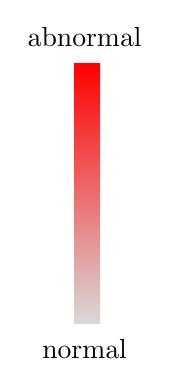
\begin{tikzpicture}[scale=1.1,auto,swap]
    \shade[top color=red,bottom color=gray!30] (0,0) rectangle (0.5,5);
    \node[inner sep=0] (corr_text) at (0.2,5.5) {abnormal};
    \node[inner sep=0] (corr_text) at (0.2,-0.5) {normal};
  \end{tikzpicture}
  \caption{}
  \label{fig:SnapEBMPCAa}
  \end{subfigure}
  
  \begin{subfigure}{1\textwidth}
  \centering
  \includegraphics[scale=0.6]{\snapLocationPCA/../patientStages.eps}
  \caption{}
  \label{fig:SnapEBMPCAb}
  \end{subfigure}

  \captionSnapEBMPCA
  
\end{figure}




\subsection{Discussion}

The EBM abnormality ordering confirms our original hypothesis, where showing that posterior regions such as occipital and superior parietal areas are the earliest to become abnormal, followed by temporal areas and inferior parietal. Moreover, in the staging histogram most controls are placed at stage zero, suggesting they have no abnormalities while PCA subjects are spread across the other stages. 

\section{AD Analysis}
\label{ebm:ad}

% \subsection{Background}
% Summarise what has been reported so far in the literature
%TODO

\subsection{Hypothesis}

In a similar way to \ref{ebm:pca}, we are interested to find out the progression of tAD using the event-based model. Previous literature has shown that the hippocampus, entorhinal cortex and other temporal areas are the first brain regions to become affected in AD \cite{braak1991neuropathological,convit1995hippocampal,xu2000usefulness}. We are interested to test this hypothesis and further find out a fine-grained picture of progression in typical AD.  

\subsection{Method}
\label{ebm:adMethod}

For doing this analysis, we used the EBM on the healthy control and tAD data from the DRC dataset. The method is exactly the same as the PCA analysis described in section \ref{ebm:pcaMethod}. 


\subsection{Results}

The results for the tAD progression are shown in Fig. \ref{fig:SnapEBMAD}. In subfigure \ref{fig:SnapEBMADa} we show the order in which cortical brain regions are affected at several stages of the EBM, according to our model. White regions are not yet affected while red regions are affected at the corresponding stage. The model assumes that all regions will eventually be affected by the disease. Moreover, in subfigure \ref{fig:SnapEBMADb} we show the histogram of EBM stages for controls and tAD subjects. 

\newcommand*{\snapLocationAD}{images/ebm/mriAllGaussUnifDirAD/snapshots} % or ../code/figures/mriAllGaussUnifDirPCA/snapshots
\newcommand*{\captionSnapEBMAD}{\caption{(a) Timing of atrophy in AD subjects according to the Event-based Model. White regions have not been affected, while red regions have been affected by the corresponding stage. (b) The histogram of EBM stages for controls and AD subjects.}\label{fig:SnapEBMAD}}


%col{x}{y}{z} respresents the color for ball z from matrix x at stage y (matrix x, stage y, ball z)
 
\definecolor{light-gray}{gray}{0.6}
\begin{figure}

  \begin{subfigure}{\textwidth}
  \centering
  %\begin{subfigure}[b]{0.15\textwidth}
    \begin{tikzpicture}[scale=1.0,auto,swap]

    % the two brain figures on top
    \node (upper_brain) at (0,1.5) { \includegraphics*[scale=\scaleBrainImg,trim=0 0 240 0]{\snapLocationAD/stage_8.eps}};
    \node (lower_brain) at (0,-1.5) { \includegraphics*[scale=\scaleBrainImg,trim=240 0 0 0]{\snapLocationAD/stage_8.eps}};
    \node[above=0cm of upper_brain] (stage) {Stage 8};
    % the balls
    
    \end{tikzpicture}
  %\end{subfigure}
  % next subfigure
  \hspace{-1.5em}
  ~
  %\begin{subfigure}[b]{0.15\textwidth}
    \begin{tikzpicture}[scale=1.0,auto,swap]

    % the two brain figures on top
    \node (upper_brain) at (0,1.5) { \includegraphics*[scale=\scaleBrainImg,trim=0 0 240 0]{\snapLocationAD/stage_16.eps}};
    \node (lower_brain) at (0,-1.5) { \includegraphics*[scale=\scaleBrainImg,trim=240 0 0 0]{\snapLocationAD/stage_16.eps}};
    \node[above=0cm of upper_brain] (stage) {Stage 16};
    % the balls
    
    \end{tikzpicture}
  %\end{subfigure}
  % next subfigure
  \hspace{-1.5em}
  ~
  %\begin{subfigure}[b]{0.15\textwidth}
    \begin{tikzpicture}[scale=1.0,auto,swap]

    % the two brain figures on top
    \node (upper_brain) at (0,1.5) { \includegraphics*[scale=\scaleBrainImg,trim=0 0 240 0]{\snapLocationAD/stage_24.eps}};
    \node (lower_brain) at (0,-1.5) { \includegraphics*[scale=\scaleBrainImg,trim=240 0 0 0]{\snapLocationAD/stage_24.eps}};
    \node[above=0cm of upper_brain] (stage) {Stage 24};
    % the balls
    
    \end{tikzpicture}
  %\end{subfigure}
  % next subfigure
  \hspace{-1.5em}
  ~
  %\begin{subfigure}[b]{0.15\textwidth}
    \begin{tikzpicture}[scale=1.0,auto,swap]

    % the two brain figures on top
    \node (upper_brain) at (0,1.5) { \includegraphics*[scale=\scaleBrainImg,trim=0 0 240 0]{\snapLocationAD/stage_32.eps}};
    \node (lower_brain) at (0,-1.5) { \includegraphics*[scale=\scaleBrainImg,trim=240 0 0 0]{\snapLocationAD/stage_32.eps}};
    \node[above=0cm of upper_brain] (stage) {Stage 32};
    % the balls
    
    \end{tikzpicture}
  %\end{subfigure}
  % next subfigure
  \hspace{-1.5em}
  ~
  %\begin{subfigure}[b]{0.15\textwidth}
    \begin{tikzpicture}[scale=1.0,auto,swap]

    % the two brain figures on top
    \node (upper_brain) at (0,1.5) { \includegraphics*[scale=\scaleBrainImg,trim=0 0 240 0]{\snapLocationAD/stage_40.eps}};
    \node (lower_brain) at (0,-1.5) { \includegraphics*[scale=\scaleBrainImg,trim=240 0 0 0]{\snapLocationAD/stage_40.eps}};
    \node[above=0cm of upper_brain] (stage) {Stage 40};
    % the balls
    
    \end{tikzpicture}
  %\end{subfigure}
  % next subfigure
  \hspace{-1.5em}
  ~
  \hspace{1em}
  % the red-to-yellow gradient on the right
  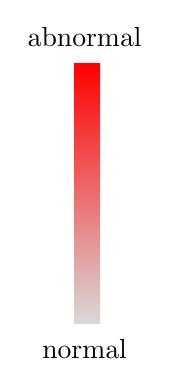
\begin{tikzpicture}[scale=1.1,auto,swap]
    \shade[top color=red,bottom color=gray!30] (0,0) rectangle (0.5,5);
    \node[inner sep=0] (corr_text) at (0.2,5.5) {abnormal};
    \node[inner sep=0] (corr_text) at (0.2,-0.5) {normal};
  \end{tikzpicture}
  \caption{}
  \label{fig:SnapEBMADa}
  \end{subfigure}
  
  \begin{subfigure}{1\textwidth}
  \centering
  \includegraphics[scale=0.6]{\snapLocationAD/../patientStages.eps}
  \caption{}
  \label{fig:SnapEBMADb}
  \end{subfigure}

  \captionSnapEBMAD
  
\end{figure}




\subsection{Discussion}
The tAD progression obtained by our data-driven model confirms previous patterns of atrophy, where the hippocampus, entorhinal, amygdala (not shown) are the earliest regions to become abnormal on in the disease time course. This is followed by other regions in this order: inferior and middle temporal regions, occipital regions, angular gyrus, precuneus and ventricles. The patient staging histogram also shows that controls are mostly at stage zero (no abnormal regions), while patients are spread across the disease stages.

\section{PCA subgroups}
\label{ebm:pca_subgroups}

\subsection{Background}

% Summarise what has been reported so far in the literature
Although PCA is considered a homogeneous disease, there have been claims in past literature that there exist three main subgroups\cite{lehmann2011basic}: parietal (dorsal) and occipitotemporal (ventral) forms of PCA have been reported by Ross et al. \cite{ross1996progressive}, while a third primary visual (striate cortex, caudal) form of PCA has been proposed by Galton et al. \cite{galton2000atypical}. In this section we are interested to analyse and compare the progression of these different subgroups. 

We split our dataset into three groups based on performance on a suite of cognitive tests. For each subject we computed the following composite tests by summing up scores from individual tests:
\begin{enumerate}
 \item Early visual processing: shape discrimination, figure-ground discrimination and simple crowding
 \item Visuoperceptual processing: object decision, fragmented letters and usual and unusual views.
 \item Visuospatial processing: number location, dot counting and a cancellation time (cut off at 90s)
 \item Episodic memory: short recognition memory test (sRMT) for words and sRMT for faces
\end{enumerate}
We then classified the subjects into three groups. The worst 1/3 of subjects on the early visual processing tests as compared to the memory tests (i.e. difference between early visual and memory tests) were assigned to the \emph{vision subgroup}. The remaining 2/3 of participants were split into two groups according to a worse performance on the visuoperceptual or visuospatial tests. More precisely, the difference between visuoperceptual and visuospatial was computed and the top half of participants was assigned to the \emph{spatial subgroup}, while the bottom half was assigned to the \emph{object subgroup}. Detailed demographics for the three PCA subgroups are shown in table \ref{tab:subgroup_demographics}.

\begin{table}
\centering
\begin{tabular}{ c |C{1.7cm} | C{1.7cm} | C{2.5cm} | C{2.5cm} | C{2.5cm}} 
\textbf{Subgroup} & \textbf{Number of Subjects} & \textbf{Gender} \hspace{1cm} M/F & \textbf{Age at baseline} \hspace{1cm} (years, mean $\pm$ std) & \textbf{Years from onset} (years, mean $\pm$ std) & \textbf{Number of scans} (mean $\pm$ std)\\
\textbf{Vision} & 23 & 6/17 & 64.4 $\pm$ 7.7 & 4.5 $\pm$ 2.8 & 2.2 $\pm$ 1.1\\ 
\textbf{Space} & 21 & 10/11 & 62.0 $\pm$ 6.8 & 4.4 $\pm$ 2.8 & 2.4 $\pm$ 1.4\\ 
\textbf{Object} & 18 & 7/11 & 62.3 $\pm$ 8.2 & 4.5 $\pm$ 2.7 & 2.7 $\pm$ 1.6\\ 
\end{tabular}
\caption[Baseline population demographics for PCA subgroups]{Baseline population demographics for PCA subgroups.}
\label{tab:subgroup_demographics}
\end{table}
 
\subsection{Hypotheses}

We formulate the following hypotheses, based on evidence from previous research\cite{ross1996progressive,galton2000atypical}:
\begin{itemize}
 \item \emph{Vision subgroup}: atrophy starts in the occipital lobe
 \item \emph{Space subgroup}: atrophy starts in the superior parietal lobe
 \item \emph{Object subgroup}: atrophy starts in the inferior temporal lobe
\end{itemize}

\subsection{Method}

We ran the EBM on data from each of the three subgroups separately, along with the shared healthy controls population. We used the same method as in the PCA analysis described in section \ref{ebm:pcaMethod}. The only difference is that we increased the range of the uniform distribution to make it span a wider interval. This was done because, due to the use of a gaussian and uniform mixture of distributions, some controls with "very good" biomarker values would be assigned to the abnormal group and subsequently later stages. Therefore, for each of the groups (\emph{vision}, \emph{space}, \emph{object}), we multiplied the initial range of the uniform distribution by a factor of 2,5 and 1 respectively.

\subsection{Results}


The positional variance matrix for the three subgroups (\emph{vision}, \emph{space}, \emph{object}) are shown in figures \ref{fig:EAR}, \ref{fig:SPA} and \ref{fig:PER} respectively. On the y-axis, we show the biomarkers representing ROI volumes ordered according to the maximum likelihood sequence $S$ from Eq. \ref{eq:ebm4}, while on the x-axis we show the position at which they become abnormal in the sequence. Each gray square at position $(i,j)$ gives the probability that biomarker $i$ is placed on position $j$ in the sequence, ranging from 0 (white cells) and to 1 (black cells).

\subsection{Discussion}

For the \emph{vision subgroup}, our hypothesis is confirmed, as the EBM suggests that the superior occipital, occipital fusiform and inferior occipital areas are the first to be affected (in no particular order). This is followed by the whole brain and parietal areas (superior parietal and precuneus). This is further followed by angular, middle occipital and middle temporal. 

In the \emph{space subgroup}, we find that the superior parietal lobe and the inferior occipital gyrus become abnormal first, again confirming our initial hypothesis. This is then followed by atrophy in the middle occipital, middle temporal, occipital fusiform and angular regions. Moreover, atrophy in the whole brain becomes detectable at this stage. 

In the \emph{object subgroup}, we find that the first two regions to become affected are the inferior occipital gyrus and the ventricles, which does not match out initial hypothesis that the inferior temporal region is affected at the very beginning. However, the inferior temporal regions is affected right after, which is still early on in the sequence. The fact that the occipital regions are also affected in this subgroup was also confirmed by previous studies \cite{ross1996progressive,kiyosawa1989alzheimer}. 


% slightly better with higher delta ... frontal went to the end but supramarginal is still at the beginning.
\begin{figure}[H]
 \centering
%  \hspace{-2.5cm}
 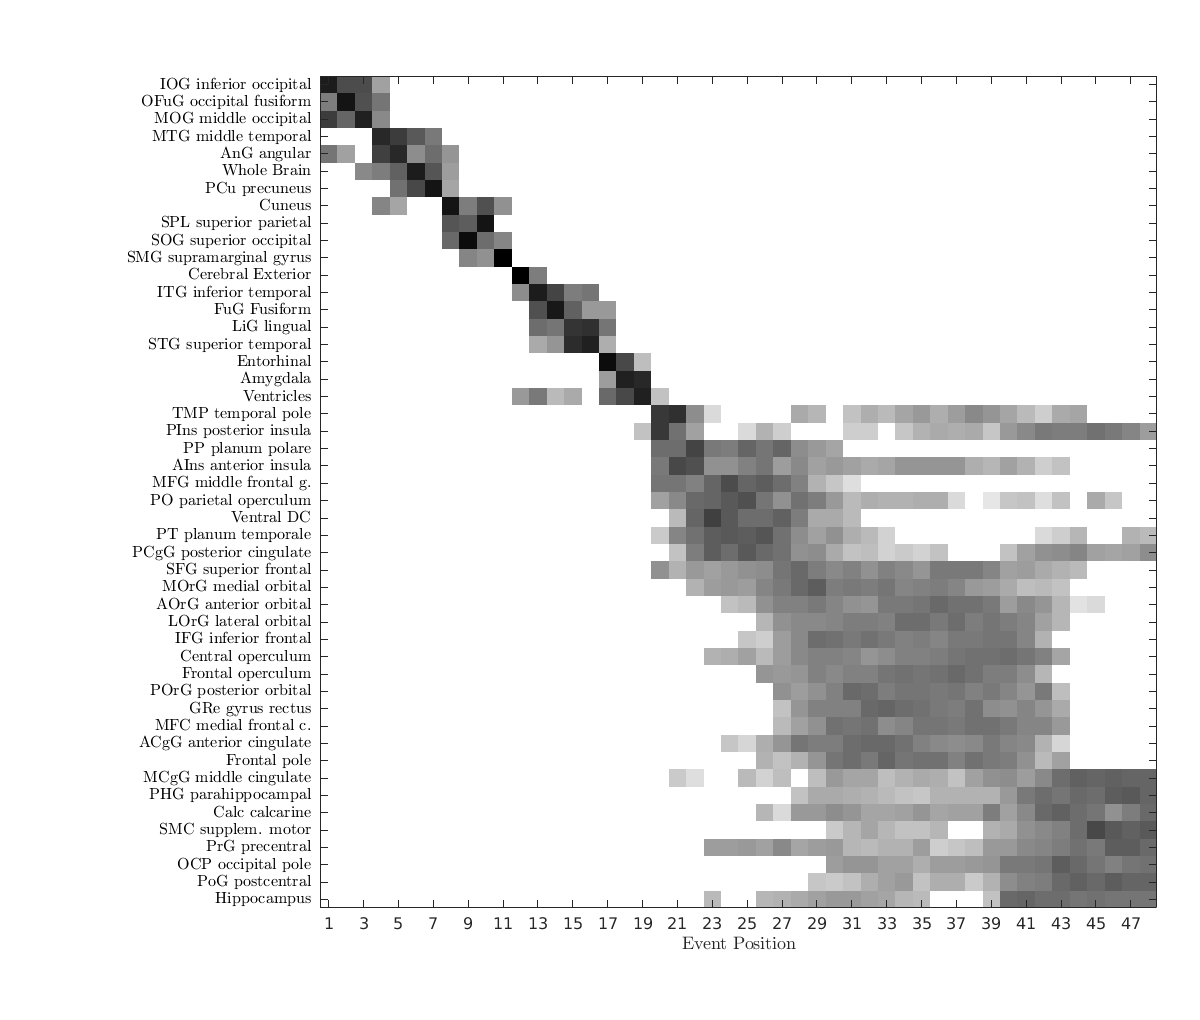
\includegraphics[scale=0.4, trim=100 50 0 0]{images/ebm/mriAllGaussUnifDirEAR/posVarianceMatrix.png}
 \caption{Positional variance matrix for the \emph{vision subgroup}. On the y-axis, we show the biomarkers representing ROI volumes ordered according to the maximum likelihood sequence, while on the x-axis we show the position at which they become abnormal in the sequence. Each gray square at position $(i,j)$ gives the probability that biomarker $i$ is placed on position $j$ in the sequence, ranging from 0 (white cells) and to 1 (black cells). Our initial hypothesis was that atrophy starts in the occipital lobe, which is confirmed by the EBM analysis.}
   \label{fig:EAR}
\end{figure}

\newcommand*{\snapLocationEAR}{images/ebm/mriAllGaussUnifDirEAR/snapshots}
\newcommand*{\captionSnapEBMEAR}{\caption{(a) Timing of atrophy for the \emph{vision} subgroup. White regions have not been affected, while red regions have been affected by the corresponding stage.}\label{fig:SnapEBMEAR}}

 
\definecolor{light-gray}{gray}{0.6}
\begin{figure}[H]
  \centering
  %\begin{subfigure}[b]{0.15\textwidth}
    \begin{tikzpicture}[scale=1.0,auto,swap]

    % the two brain figures on top
    \node (upper_brain) at (0,1.5) { \includegraphics*[scale=\scaleBrainImg,trim=0 0 240 0]{\snapLocationEAR/stage_1.eps}};
    \node (lower_brain) at (0,-1.5) { \includegraphics*[scale=\scaleBrainImg,trim=240 0 0 0]{\snapLocationEAR/stage_1.eps}};
    \node[above=0cm of upper_brain] (stage) {Stage 1};
    % the balls
    
    \end{tikzpicture}
  %\end{subfigure}
  % next subfigure
  \hspace{-1.5em}
  ~
  %\begin{subfigure}[b]{0.15\textwidth}
    \begin{tikzpicture}[scale=1.0,auto,swap]

    % the two brain figures on top
    \node (upper_brain) at (0,1.5) { \includegraphics*[scale=\scaleBrainImg,trim=0 0 240 0]{\snapLocationEAR/stage_2.eps}};
    \node (lower_brain) at (0,-1.5) { \includegraphics*[scale=\scaleBrainImg,trim=240 0 0 0]{\snapLocationEAR/stage_2.eps}};
    \node[above=0cm of upper_brain] (stage) {Stage 2};
    % the balls
    
    \end{tikzpicture}
  %\end{subfigure}
  % next subfigure
  \hspace{-1.5em}
  ~
  %\begin{subfigure}[b]{0.15\textwidth}
    \begin{tikzpicture}[scale=1.0,auto,swap]

    % the two brain figures on top
    \node (upper_brain) at (0,1.5) { \includegraphics*[scale=\scaleBrainImg,trim=0 0 240 0]{\snapLocationEAR/stage_3.eps}};
    \node (lower_brain) at (0,-1.5) { \includegraphics*[scale=\scaleBrainImg,trim=240 0 0 0]{\snapLocationEAR/stage_3.eps}};
    \node[above=0cm of upper_brain] (stage) {Stage 3};
    % the balls
    
    \end{tikzpicture}
  %\end{subfigure}
  % next subfigure
  \hspace{-1.5em}
  ~
  %\begin{subfigure}[b]{0.15\textwidth}
    \begin{tikzpicture}[scale=1.0,auto,swap]

    % the two brain figures on top
    \node (upper_brain) at (0,1.5) { \includegraphics*[scale=\scaleBrainImg,trim=0 0 240 0]{\snapLocationEAR/stage_4.eps}};
    \node (lower_brain) at (0,-1.5) { \includegraphics*[scale=\scaleBrainImg,trim=240 0 0 0]{\snapLocationEAR/stage_4.eps}};
    \node[above=0cm of upper_brain] (stage) {Stage 4};
    % the balls
    
    \end{tikzpicture}
  %\end{subfigure}
  % next subfigure
  \hspace{-1.5em}
  ~
  %\begin{subfigure}[b]{0.15\textwidth}
    \begin{tikzpicture}[scale=1.0,auto,swap]

    % the two brain figures on top
    \node (upper_brain) at (0,1.5) { \includegraphics*[scale=\scaleBrainImg,trim=0 0 240 0]{\snapLocationEAR/stage_5.eps}};
    \node (lower_brain) at (0,-1.5) { \includegraphics*[scale=\scaleBrainImg,trim=240 0 0 0]{\snapLocationEAR/stage_5.eps}};
    \node[above=0cm of upper_brain] (stage) {Stage 5};
    % the balls
    
    \end{tikzpicture}
  %\end{subfigure}
  % next subfigure
  \hspace{-1.5em}
  ~
  %\begin{subfigure}[b]{0.15\textwidth}
    \begin{tikzpicture}[scale=1.0,auto,swap]

    % the two brain figures on top
    \node (upper_brain) at (0,1.5) { \includegraphics*[scale=\scaleBrainImg,trim=0 0 240 0]{\snapLocationEAR/stage_6.eps}};
    \node (lower_brain) at (0,-1.5) { \includegraphics*[scale=\scaleBrainImg,trim=240 0 0 0]{\snapLocationEAR/stage_6.eps}};
    \node[above=0cm of upper_brain] (stage) {Stage 6};
    % the balls
    
    \end{tikzpicture}
  %\end{subfigure}
  % next subfigure
  \hspace{-1.5em}
  ~
  %\begin{subfigure}[b]{0.15\textwidth}
    \begin{tikzpicture}[scale=1.0,auto,swap]

    % the two brain figures on top
    \node (upper_brain) at (0,1.5) { \includegraphics*[scale=\scaleBrainImg,trim=0 0 240 0]{\snapLocationEAR/stage_7.eps}};
    \node (lower_brain) at (0,-1.5) { \includegraphics*[scale=\scaleBrainImg,trim=240 0 0 0]{\snapLocationEAR/stage_7.eps}};
    \node[above=0cm of upper_brain] (stage) {Stage 7};
    % the balls
    
    \end{tikzpicture}
  %\end{subfigure}
  % next subfigure
  \hspace{-1.5em}
  ~
  %\begin{subfigure}[b]{0.15\textwidth}
    \begin{tikzpicture}[scale=1.0,auto,swap]

    % the two brain figures on top
    \node (upper_brain) at (0,1.5) { \includegraphics*[scale=\scaleBrainImg,trim=0 0 240 0]{\snapLocationEAR/stage_8.eps}};
    \node (lower_brain) at (0,-1.5) { \includegraphics*[scale=\scaleBrainImg,trim=240 0 0 0]{\snapLocationEAR/stage_8.eps}};
    \node[above=0cm of upper_brain] (stage) {Stage 8};
    % the balls
    
    \end{tikzpicture}
  %\end{subfigure}
  % next subfigure
  \hspace{-1.5em}
  ~
  %\begin{subfigure}[b]{0.15\textwidth}
    \begin{tikzpicture}[scale=1.0,auto,swap]

    % the two brain figures on top
    \node (upper_brain) at (0,1.5) { \includegraphics*[scale=\scaleBrainImg,trim=0 0 240 0]{\snapLocationEAR/stage_9.eps}};
    \node (lower_brain) at (0,-1.5) { \includegraphics*[scale=\scaleBrainImg,trim=240 0 0 0]{\snapLocationEAR/stage_9.eps}};
    \node[above=0cm of upper_brain] (stage) {Stage 9};
    % the balls
    
    \end{tikzpicture}
  %\end{subfigure}
  % next subfigure
  \hspace{-1.5em}
  ~
  \hspace{1em}
  % the red-to-yellow gradient on the right
  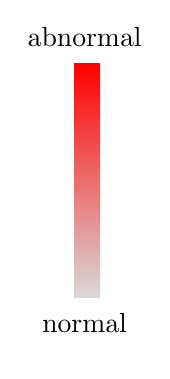
\begin{tikzpicture}[scale=1.1,auto,swap]
    \shade[top color=red,bottom color=gray!30] (0,1.5) rectangle (0.5,6);
    \node[inner sep=0] (corr_text) at (0.2,6.5) {abnormal};
    \node[inner sep=0] (corr_text) at (0.2,1) {normal};
    \node[inner sep=0] (corr_text) at (0.2,0.5) {};
  \end{tikzpicture}
  \captionSnapEBMEAR
\end{figure}





% \pagebreak

% superior parietal went earlier with around 4 positions, but still on place 4
\begin{figure}[H]
 \centering
%  \hspace{-2.5cm}
 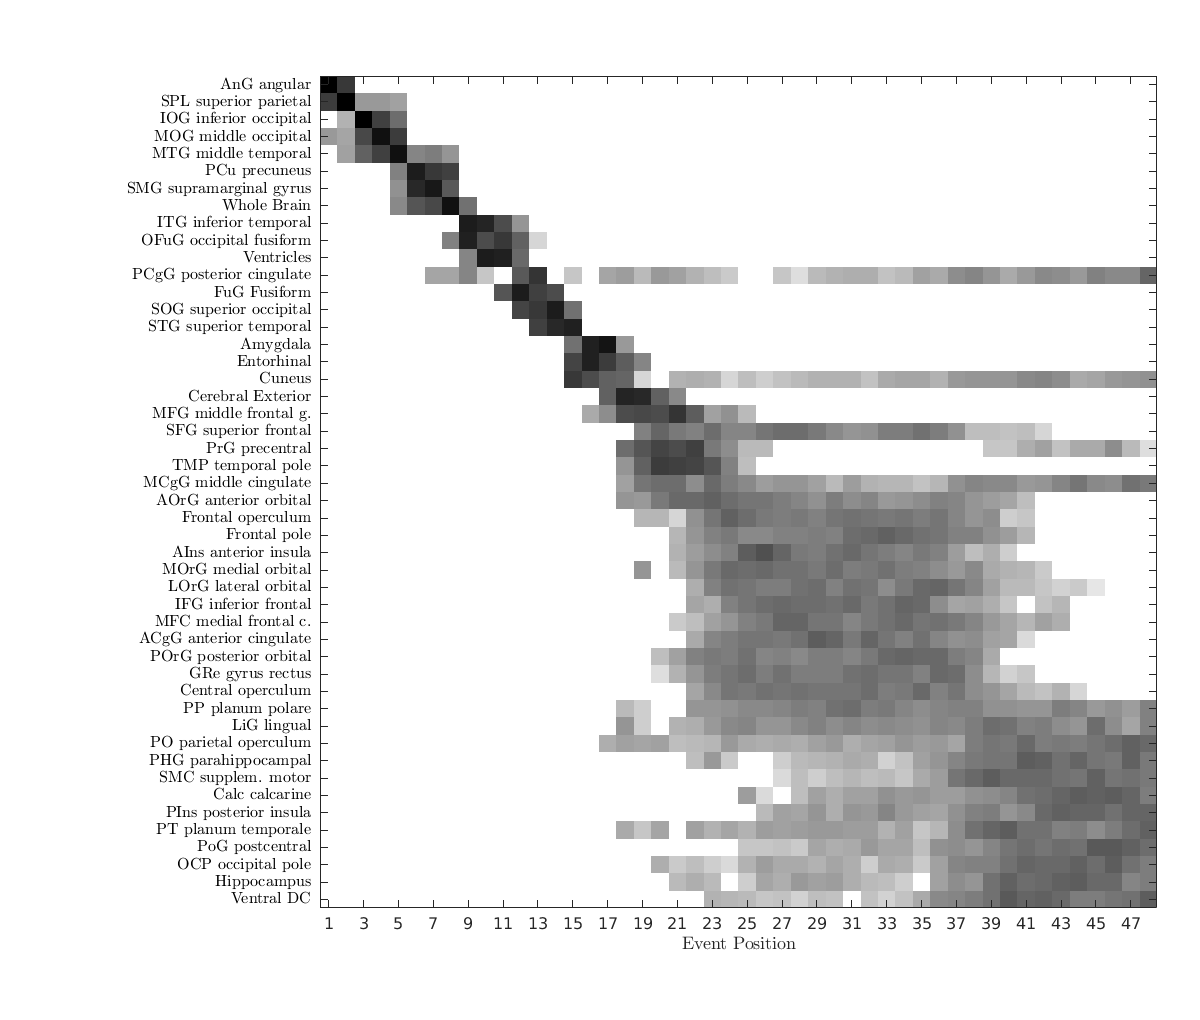
\includegraphics[scale=0.4, trim=100 50 0 0]{images/ebm/mriAllGaussUnifDirSPA/posVarianceMatrix.png}
 \caption{Positional variance matrix for the \emph{space subgroup}. On the y-axis, we show the biomarkers representing ROI volumes ordered according to the maximum likelihood sequence, while on the x-axis we show the position at which they become abnormal in the sequence. Each gray square at position $(i,j)$ gives the probability that biomarker $i$ is placed on position $j$ in the sequence, ranging from 0 (white cells) and to 1 (black cells). Our initial hypothesis was that atrophy starts in the superior parietal lobe. This is confirmed by the EBM analysis, which suggests atrophy starts in the angular and superior parietal regions.}
   \label{fig:SPA}
\end{figure}

\newcommand*{\snapLocationSPA}{images/ebm/mriAllGaussUnifDirSPA/snapshots} 
\newcommand*{\captionSnapEBMSPA}{\caption{(a) Timing of atrophy for the \emph{space} subgroup. White regions have not been affected, while red regions have been affected by the corresponding stage.}\label{fig:SnapEBMSPA}}


 
\definecolor{light-gray}{gray}{0.6}
\begin{figure}[H]
  \centering
  %\begin{subfigure}[b]{0.15\textwidth}
    \begin{tikzpicture}[scale=1.0,auto,swap]

    % the two brain figures on top
    \node (upper_brain) at (0,1.5) { \includegraphics*[scale=\scaleBrainImg,trim=0 0 240 0]{\snapLocationSPA/stage_1.eps}};
    \node (lower_brain) at (0,-1.5) { \includegraphics*[scale=\scaleBrainImg,trim=240 0 0 0]{\snapLocationSPA/stage_1.eps}};
    \node[above=0cm of upper_brain] (stage) {Stage 1};
    % the balls
    
    \end{tikzpicture}
  %\end{subfigure}
  % next subfigure
  \hspace{-1.5em}
  ~
  %\begin{subfigure}[b]{0.15\textwidth}
    \begin{tikzpicture}[scale=1.0,auto,swap]

    % the two brain figures on top
    \node (upper_brain) at (0,1.5) { \includegraphics*[scale=\scaleBrainImg,trim=0 0 240 0]{\snapLocationSPA/stage_2.eps}};
    \node (lower_brain) at (0,-1.5) { \includegraphics*[scale=\scaleBrainImg,trim=240 0 0 0]{\snapLocationSPA/stage_2.eps}};
    \node[above=0cm of upper_brain] (stage) {Stage 2};
    % the balls
    
    \end{tikzpicture}
  %\end{subfigure}
  % next subfigure
  \hspace{-1.5em}
  ~
  %\begin{subfigure}[b]{0.15\textwidth}
    \begin{tikzpicture}[scale=1.0,auto,swap]

    % the two brain figures on top
    \node (upper_brain) at (0,1.5) { \includegraphics*[scale=\scaleBrainImg,trim=0 0 240 0]{\snapLocationSPA/stage_3.eps}};
    \node (lower_brain) at (0,-1.5) { \includegraphics*[scale=\scaleBrainImg,trim=240 0 0 0]{\snapLocationSPA/stage_3.eps}};
    \node[above=0cm of upper_brain] (stage) {Stage 3};
    % the balls
    
    \end{tikzpicture}
  %\end{subfigure}
  % next subfigure
  \hspace{-1.5em}
  ~
  %\begin{subfigure}[b]{0.15\textwidth}
    \begin{tikzpicture}[scale=1.0,auto,swap]

    % the two brain figures on top
    \node (upper_brain) at (0,1.5) { \includegraphics*[scale=\scaleBrainImg,trim=0 0 240 0]{\snapLocationSPA/stage_4.eps}};
    \node (lower_brain) at (0,-1.5) { \includegraphics*[scale=\scaleBrainImg,trim=240 0 0 0]{\snapLocationSPA/stage_4.eps}};
    \node[above=0cm of upper_brain] (stage) {Stage 4};
    % the balls
    
    \end{tikzpicture}
  %\end{subfigure}
  % next subfigure
  \hspace{-1.5em}
  ~
  %\begin{subfigure}[b]{0.15\textwidth}
    \begin{tikzpicture}[scale=1.0,auto,swap]

    % the two brain figures on top
    \node (upper_brain) at (0,1.5) { \includegraphics*[scale=\scaleBrainImg,trim=0 0 240 0]{\snapLocationSPA/stage_5.eps}};
    \node (lower_brain) at (0,-1.5) { \includegraphics*[scale=\scaleBrainImg,trim=240 0 0 0]{\snapLocationSPA/stage_5.eps}};
    \node[above=0cm of upper_brain] (stage) {Stage 5};
    % the balls
    
    \end{tikzpicture}
  %\end{subfigure}
  % next subfigure
  \hspace{-1.5em}
  ~
  %\begin{subfigure}[b]{0.15\textwidth}
    \begin{tikzpicture}[scale=1.0,auto,swap]

    % the two brain figures on top
    \node (upper_brain) at (0,1.5) { \includegraphics*[scale=\scaleBrainImg,trim=0 0 240 0]{\snapLocationSPA/stage_6.eps}};
    \node (lower_brain) at (0,-1.5) { \includegraphics*[scale=\scaleBrainImg,trim=240 0 0 0]{\snapLocationSPA/stage_6.eps}};
    \node[above=0cm of upper_brain] (stage) {Stage 6};
    % the balls
    
    \end{tikzpicture}
  %\end{subfigure}
  % next subfigure
  \hspace{-1.5em}
  ~
  %\begin{subfigure}[b]{0.15\textwidth}
    \begin{tikzpicture}[scale=1.0,auto,swap]

    % the two brain figures on top
    \node (upper_brain) at (0,1.5) { \includegraphics*[scale=\scaleBrainImg,trim=0 0 240 0]{\snapLocationSPA/stage_7.eps}};
    \node (lower_brain) at (0,-1.5) { \includegraphics*[scale=\scaleBrainImg,trim=240 0 0 0]{\snapLocationSPA/stage_7.eps}};
    \node[above=0cm of upper_brain] (stage) {Stage 7};
    % the balls
    
    \end{tikzpicture}
  %\end{subfigure}
  % next subfigure
  \hspace{-1.5em}
  ~
  %\begin{subfigure}[b]{0.15\textwidth}
    \begin{tikzpicture}[scale=1.0,auto,swap]

    % the two brain figures on top
    \node (upper_brain) at (0,1.5) { \includegraphics*[scale=\scaleBrainImg,trim=0 0 240 0]{\snapLocationSPA/stage_8.eps}};
    \node (lower_brain) at (0,-1.5) { \includegraphics*[scale=\scaleBrainImg,trim=240 0 0 0]{\snapLocationSPA/stage_8.eps}};
    \node[above=0cm of upper_brain] (stage) {Stage 8};
    % the balls
    
    \end{tikzpicture}
  %\end{subfigure}
  % next subfigure
  \hspace{-1.5em}
  ~
  %\begin{subfigure}[b]{0.15\textwidth}
    \begin{tikzpicture}[scale=1.0,auto,swap]

    % the two brain figures on top
    \node (upper_brain) at (0,1.5) { \includegraphics*[scale=\scaleBrainImg,trim=0 0 240 0]{\snapLocationSPA/stage_9.eps}};
    \node (lower_brain) at (0,-1.5) { \includegraphics*[scale=\scaleBrainImg,trim=240 0 0 0]{\snapLocationSPA/stage_9.eps}};
    \node[above=0cm of upper_brain] (stage) {Stage 9};
    % the balls
    
    \end{tikzpicture}
  %\end{subfigure}
  % next subfigure
  \hspace{-1.5em}
  ~
  \hspace{1em}
  % the red-to-yellow gradient on the right
  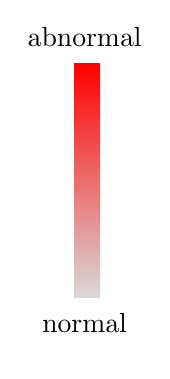
\begin{tikzpicture}[scale=1.1,auto,swap]
    \shade[top color=red,bottom color=gray!30] (0,1.5) rectangle (0.5,6);
    \node[inner sep=0] (corr_text) at (0.2,6.5) {abnormal};
    \node[inner sep=0] (corr_text) at (0.2,1) {normal};
    \node[inner sep=0] (corr_text) at (0.2,0.5) {};
  \end{tikzpicture}
  \captionSnapEBMSPA
\end{figure}





% \pagebreak

\begin{figure}[H]
 \centering
%  \hspace{-2.5cm}
 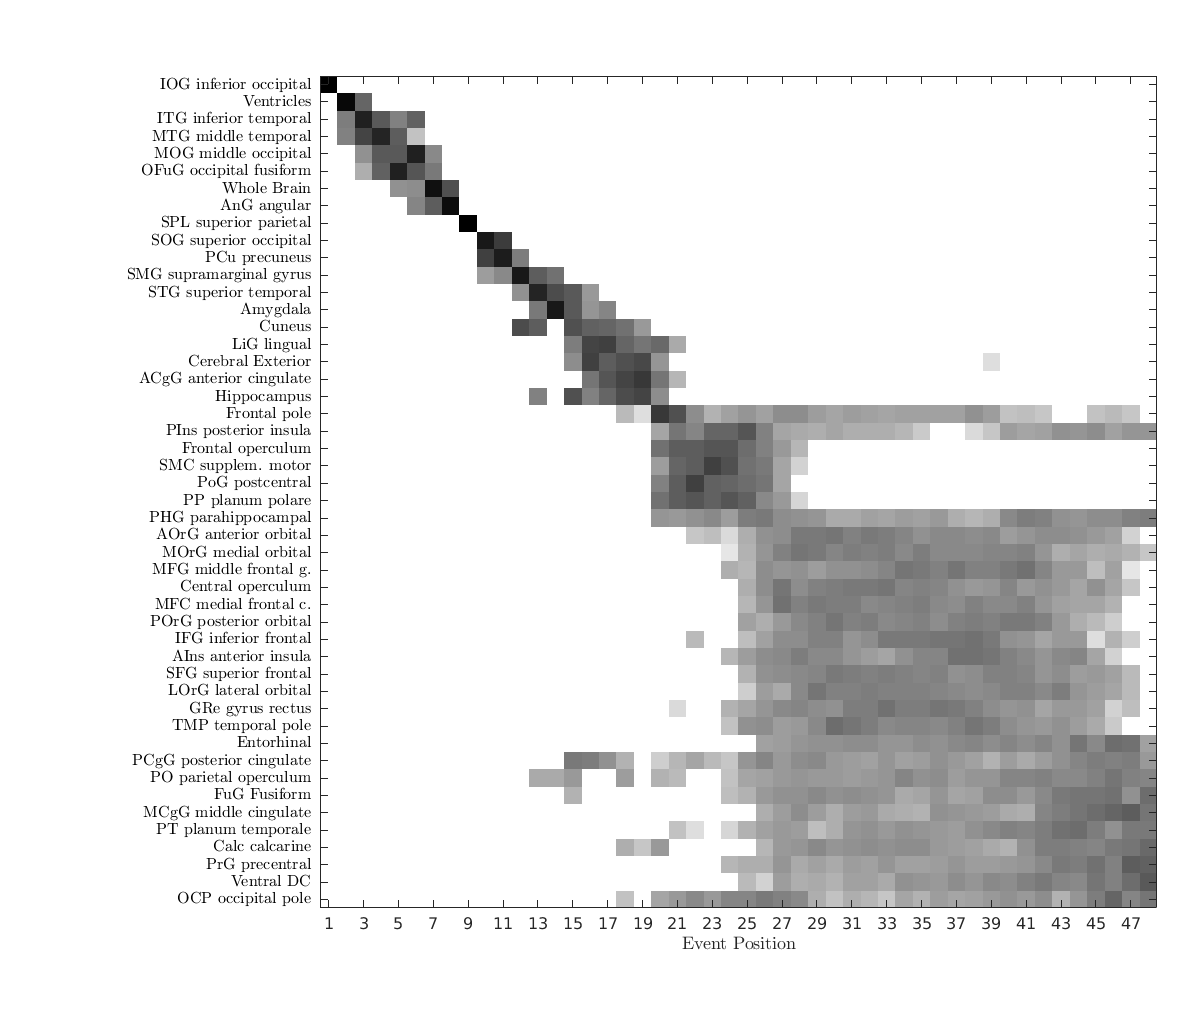
\includegraphics[scale=0.4, trim=100 50 0 0]{images/ebm/mriAllGaussUnifDirPER/posVarianceMatrix.png}
 \caption{Positional variance matrix for the \emph{object subgroup}. On the y-axis, we show the biomarkers representing ROI volumes ordered according to the maximum likelihood sequence, while on the x-axis we show the position at which they become abnormal in the sequence. Each gray square at position $(i,j)$ gives the probability that biomarker $i$ is placed on position $j$ in the sequence, ranging from 0 (white cells) and to 1 (black cells). Our initial hypothesis was that atrophy starts in the inferior temporal lobe, which is not confirmed by the EBM analysis as the inferior temporal region becomes abnormal only after the inferior occipital and ventricles.}
   \label{fig:PER}
\end{figure}

\newcommand*{\snapLocationPER}{images/ebm/mriAllGaussUnifDirPER/snapshots} % 
\newcommand*{\captionSnapEBMPER}{\caption{(a) Timing of atrophy for the \emph{object} subgroup. White regions have not been affected, while red regions have been affected by the corresponding stage.}\label{fig:SnapEBMPER}}


 
\definecolor{light-gray}{gray}{0.6}
\begin{figure}[H]
  \centering
  %\begin{subfigure}[b]{0.15\textwidth}
    \begin{tikzpicture}[scale=1.0,auto,swap]

    % the two brain figures on top
    \node (upper_brain) at (0,1.5) { \includegraphics*[scale=\scaleBrainImg,trim=0 0 240 0]{\snapLocationPER/stage_1.eps}};
    \node (lower_brain) at (0,-1.5) { \includegraphics*[scale=\scaleBrainImg,trim=240 0 0 0]{\snapLocationPER/stage_1.eps}};
    \node[above=0cm of upper_brain] (stage) {Stage 1};
    % the balls
    
    \end{tikzpicture}
  %\end{subfigure}
  % next subfigure
  \hspace{-1.5em}
  ~
  %\begin{subfigure}[b]{0.15\textwidth}
    \begin{tikzpicture}[scale=1.0,auto,swap]

    % the two brain figures on top
    \node (upper_brain) at (0,1.5) { \includegraphics*[scale=\scaleBrainImg,trim=0 0 240 0]{\snapLocationPER/stage_2.eps}};
    \node (lower_brain) at (0,-1.5) { \includegraphics*[scale=\scaleBrainImg,trim=240 0 0 0]{\snapLocationPER/stage_2.eps}};
    \node[above=0cm of upper_brain] (stage) {Stage 2};
    % the balls
    
    \end{tikzpicture}
  %\end{subfigure}
  % next subfigure
  \hspace{-1.5em}
  ~
  %\begin{subfigure}[b]{0.15\textwidth}
    \begin{tikzpicture}[scale=1.0,auto,swap]

    % the two brain figures on top
    \node (upper_brain) at (0,1.5) { \includegraphics*[scale=\scaleBrainImg,trim=0 0 240 0]{\snapLocationPER/stage_3.eps}};
    \node (lower_brain) at (0,-1.5) { \includegraphics*[scale=\scaleBrainImg,trim=240 0 0 0]{\snapLocationPER/stage_3.eps}};
    \node[above=0cm of upper_brain] (stage) {Stage 3};
    % the balls
    
    \end{tikzpicture}
  %\end{subfigure}
  % next subfigure
  \hspace{-1.5em}
  ~
  %\begin{subfigure}[b]{0.15\textwidth}
    \begin{tikzpicture}[scale=1.0,auto,swap]

    % the two brain figures on top
    \node (upper_brain) at (0,1.5) { \includegraphics*[scale=\scaleBrainImg,trim=0 0 240 0]{\snapLocationPER/stage_4.eps}};
    \node (lower_brain) at (0,-1.5) { \includegraphics*[scale=\scaleBrainImg,trim=240 0 0 0]{\snapLocationPER/stage_4.eps}};
    \node[above=0cm of upper_brain] (stage) {Stage 4};
    % the balls
    
    \end{tikzpicture}
  %\end{subfigure}
  % next subfigure
  \hspace{-1.5em}
  ~
  %\begin{subfigure}[b]{0.15\textwidth}
    \begin{tikzpicture}[scale=1.0,auto,swap]

    % the two brain figures on top
    \node (upper_brain) at (0,1.5) { \includegraphics*[scale=\scaleBrainImg,trim=0 0 240 0]{\snapLocationPER/stage_5.eps}};
    \node (lower_brain) at (0,-1.5) { \includegraphics*[scale=\scaleBrainImg,trim=240 0 0 0]{\snapLocationPER/stage_5.eps}};
    \node[above=0cm of upper_brain] (stage) {Stage 5};
    % the balls
    
    \end{tikzpicture}
  %\end{subfigure}
  % next subfigure
  \hspace{-1.5em}
  ~
  %\begin{subfigure}[b]{0.15\textwidth}
    \begin{tikzpicture}[scale=1.0,auto,swap]

    % the two brain figures on top
    \node (upper_brain) at (0,1.5) { \includegraphics*[scale=\scaleBrainImg,trim=0 0 240 0]{\snapLocationPER/stage_6.eps}};
    \node (lower_brain) at (0,-1.5) { \includegraphics*[scale=\scaleBrainImg,trim=240 0 0 0]{\snapLocationPER/stage_6.eps}};
    \node[above=0cm of upper_brain] (stage) {Stage 6};
    % the balls
    
    \end{tikzpicture}
  %\end{subfigure}
  % next subfigure
  \hspace{-1.5em}
  ~
  %\begin{subfigure}[b]{0.15\textwidth}
    \begin{tikzpicture}[scale=1.0,auto,swap]

    % the two brain figures on top
    \node (upper_brain) at (0,1.5) { \includegraphics*[scale=\scaleBrainImg,trim=0 0 240 0]{\snapLocationPER/stage_7.eps}};
    \node (lower_brain) at (0,-1.5) { \includegraphics*[scale=\scaleBrainImg,trim=240 0 0 0]{\snapLocationPER/stage_7.eps}};
    \node[above=0cm of upper_brain] (stage) {Stage 7};
    % the balls
    
    \end{tikzpicture}
  %\end{subfigure}
  % next subfigure
  \hspace{-1.5em}
  ~
  %\begin{subfigure}[b]{0.15\textwidth}
    \begin{tikzpicture}[scale=1.0,auto,swap]

    % the two brain figures on top
    \node (upper_brain) at (0,1.5) { \includegraphics*[scale=\scaleBrainImg,trim=0 0 240 0]{\snapLocationPER/stage_8.eps}};
    \node (lower_brain) at (0,-1.5) { \includegraphics*[scale=\scaleBrainImg,trim=240 0 0 0]{\snapLocationPER/stage_8.eps}};
    \node[above=0cm of upper_brain] (stage) {Stage 8};
    % the balls
    
    \end{tikzpicture}
  %\end{subfigure}
  % next subfigure
  \hspace{-1.5em}
  ~
  %\begin{subfigure}[b]{0.15\textwidth}
    \begin{tikzpicture}[scale=1.0,auto,swap]

    % the two brain figures on top
    \node (upper_brain) at (0,1.5) { \includegraphics*[scale=\scaleBrainImg,trim=0 0 240 0]{\snapLocationPER/stage_9.eps}};
    \node (lower_brain) at (0,-1.5) { \includegraphics*[scale=\scaleBrainImg,trim=240 0 0 0]{\snapLocationPER/stage_9.eps}};
    \node[above=0cm of upper_brain] (stage) {Stage 9};
    % the balls
    
    \end{tikzpicture}
  %\end{subfigure}
  % next subfigure
  \hspace{-1.5em}
  ~
  \hspace{1em}
  % the red-to-yellow gradient on the right
  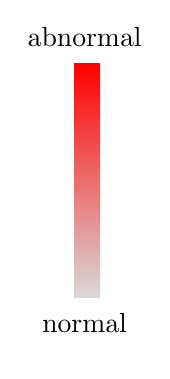
\begin{tikzpicture}[scale=1.1,auto,swap]
    \shade[top color=red,bottom color=gray!30] (0,1.5) rectangle (0.5,6);
    \node[inner sep=0] (corr_text) at (0.2,6.5) {abnormal};
    \node[inner sep=0] (corr_text) at (0.2,1) {normal};
    \node[inner sep=0] (corr_text) at (0.2,0.5) {};
  \end{tikzpicture}
  \captionSnapEBMPER
\end{figure}




\section{Conclusion}

% summary
In this chapter we showed that the EBM is a powerful tool for studying progression of typical Alzheimer disease and other subtypes. The main advantages of the model is that it does not require longitudinal data, making it especially useful for analysing rare dementias where no no large, longitudinal datasets currently exist. We have shown that the EBM results confirm patterns of atrophy previously reported in the literature, but gives a much more fine-grained picture of the temporal progression than these studies.

% limitation of the analysis (not the EBM)
The current analysis has several limitations. First of all, we assumed that the control population was well defined in order to fit the distribution of normal biomarker values directly on control data. However, the controls might show some abnormalities in CSF biomarkers, but no such data was available. Secondly, we only explored brain volumes, but other biomarkers such as cortical thickness can be further analysed using our data. 

% Future work motivated by the limitations
There are several avenues of future research. For fitting the distributions of normal and abnormal biomarker values we could use data-driven methods such as mixture model optimisation. Another option is to use the optimised EBM fitting procedures such as simultaneous sampling (section \ref{sec:simultSampling}) or Expectation-Maximisation (section \ref{sec:ebmEM}). Further analysis also needs to be done in order to answer questions related to the extent and rate of atrophy in PCA and the respective subgroups. This analysis has been done with the differential equation model in chapter \ref{chapter:diffeq}, but not at the PCA subgroup level due to the lack of sufficient longitudinal data. 

